\renewcommand{\theequation}{\theenumi}
\begin{enumerate}[label=\arabic*.,ref=\thesubsection.\theenumi]
\numberwithin{equation}{enumi}
	%
\item
	Show that if
\begin{equation}
\label{ch5_sin_increasing}
\theta_1 < \theta_2, \quad \sin \theta_1 < \sin \theta_2.
\end{equation}	
\begin{figure}[!ht]
	\begin{center}
		
		%\includegraphics[width=\columnwidth]{./figs/ch5_sin_theta}
		%\vspace*{-10cm}
		\resizebox{\columnwidth}{!}{\begin{tikzpicture}
[scale =3,>=stealth,point/.style = {draw, circle, fill = black, inner sep = 1pt},]

\node (A) at (0,3)[point,label=above :$A$] {};
\node (B) at (3,0)[point,label=below :$B$] {};
\node (C) at (0,0)[point,label=below :$C$] {};
\node (D) at (0,1.5)[point,label=left :$D$] {};
\draw (A)--(B);
\draw (C)--(B);
\draw (A)--(C);
\draw (B)--(D);
%\tkzMarkAngle[size=.4](A,B,D);
\tkzMarkAngle[size=.4](C,A,B);
%\tkzMarkAngle[size=.3](D,B,C);
\tkzMarkAngle[size=.3](C,D,B);
\tkzMarkRightAngle[size=.15](A,C,B);

\node [above] at (1.6,1.5){$c$};
\node [below] at (1.6,0){$a$};
\node [below] at (1.6,1){$l$};
\node [above] at (-0.2,1.5){$b$};
\node [above] at (-0.2,0.5){$x$};
%\node [above] at (2.5,0){$\theta_2$};
%\node [above] at (2.5,0.3){$\theta_1$};
\node [above] at (0.2,2.4){$\theta_2$};
\node [above] at (0.2,1.0){$\theta_1$};
\end{tikzpicture}
}
	\end{center}
	\caption{$\theta_1 < \theta_2 \implies \sin \theta_1 < \sin \theta_2.$}
	\label{fig:fig_sin_ineq}	
\end{figure}
%
\solution Using Baudhayana's theorem in $\triangle  ABC$ and $\triangle DBC$
%
\begin{align}
l^2 &= x^2+a^2
\\
c^2 &= b^2+a^2
\\
\implies c > l &\because b > x.
\label{eq:tri_sin_ineq_hyp}
\end{align}
%
Also, 
%
\begin{align}
a = c \sin \theta_1 &= l \sin \theta_2
%
\\
\implies 
\frac{\sin \theta_1}{\sin \theta_2} = \frac{l}{c} &< 1 \quad \text{from }\eqref{eq:tri_sin_ineq_hyp}
\\
\text{or, } {\sin \theta_1}<{\sin \theta_2}
\label{eq:tri_sin_ineq}
\end{align}
%
	%
	\item
		Show that if
		\begin{equation}
		\label{ch5_cos_decreasing}
		\theta_1 < \theta_2, \cos \theta_1 > \cos \theta_2.
		\end{equation}	
%
\item	Show that in any $\triangle ABC$, $\angle A > \angle B \implies a > b$.
%
\\
\solution Use \eqref{eq:tri_sin_form} and \eqref{eq:tri_sin_ineq}
%
\item Show that the sum of any two sides of a triangle is greater than the third side.
\\
\solution In Hero's formula in \eqref{eq:tri_hero}, all the factors inside the square root should be positive.  Thus, 
%
\begin{align}
\brak{s-a} > 0, \brak{s-b} > 0\brak{s-c} &> 0
\end{align}
%
\begin{align}
\\
\brak{s-a} > 0 \implies \frac{a+b+c}{2} -a &> 0
\\
\text{or, } b+c > a
\end{align}
%
Similarly, it can be shown that $a+b>c, c+a>b$.


	%
%\item
%	In Fig. \ref{ch3_angle_bisector}, $OB$ divides the  $\angle B$ into half, i.e.\begin{equation}
%	\angle OBC = \angle OBA
%	\end{equation}
%	$OB$ is known as an angle bisector.
%
%
%\begin{figure}[!ht]
%	\begin{center}
%		
%		%\includegraphics[width=\columnwidth]{./figs/ch3_angle_bisector}
%		%\vspace*{-10cm}
%		\resizebox{\columnwidth}{!}{\begin{tikzpicture}
[scale=2,>=stealth,point/.style={draw,circle,fill = black,inner sep=0.5pt},]

\node (D) at (0, 0)[point,label=below :$D$] {};
\node (A) at (0, 3)[point,label=above :$A$]{};
\node (B) at (-3, 0)[point,label=below left:$B$]{};
\node (C) at (3, 0)[point,label=below right:$C$]{};
\node (O) at (0, 1.3)[point,label=below right:$O$]{};
\node (F) at (-1.1, 1.9)[point,label=above left:$F$]{};
\node (E) at (1.1, 1.9)[point,label=above right:$E$]{};

\draw (D)--(B);
\draw (B)--(A);
\draw (A)--(C);
\draw (C)--(D);
\draw [thick,dashed] (A) -- (D);
\draw [thick,dashed] (O) -- (E);
\draw [thick,dashed] (O) -- (F);
\draw (B)--(O);
\draw (C)--(O);

\tkzMarkRightAngle[size=.2](A,D,C)
\tkzMarkRightAngle[size=.15](B,F,O);
\tkzMarkRightAngle[size=.15](C,E,O);
\tkzMarkAngle[size=.4](D,B,O);
\tkzMarkAngle[size=.35](O,B,F);
\tkzMarkAngle[size=.54](E,C,O);
\tkzMarkAngle[size=.5](E,C,O);
\tkzMarkAngle[size=.6](O,C,D);
\tkzMarkAngle[size=.65](O,C,D);

\end{tikzpicture}}
%	\end{center}
%	\caption{Angle bisectors meet at a point}
%	\label{ch3_angle_bisector}	
%\end{figure}
%
%	$OB$ and $OC$ are angle bisectors of angles $B$ and $C$. $OA$ is joined and $OD, OF$ and $OE$ are perpendiculars to sides $a,b$ and $c$.
%\item
%  Show that $OD = OE = OF$.
%\solution In $\Delta$s $ODC$ and $OEC$,
%\begin{align}
%OD &= OC \sin \frac{C}{2}
%\\
%OE &= OC \sin \frac{C}{2} 
%\\
%\Rightarrow OD &=OE.
%\end{align}
%Similarly,
%\begin{equation}
%OD = OF.
%\end{equation}
%%
%\item
%	Show that OA is the angle bisector of $\angle A$
%
%\solution In $\Delta$s $OFA$ and $OEA$,
%\begin{align}
%OF &= OE
%\\
%\Rightarrow OA \sin OAF &= OA \sin OAE \\
%\Rightarrow \sin OAF &=  \sin OAE \\
%\Rightarrow \angle OAF &= \angle OAE
%\end{align}
%which proves that $OA$ bisects $\angle A$.
%{\em Conclusion:} The angle bisectors of a triangle meet at a point.
%
%\end{enumerate}
%\subsection{Congruent Triangles}
%%
%\renewcommand{\theequation}{\theenumi}
%\begin{enumerate}[label=\arabic*.,ref=\thesubsection.\theenumi]
%\numberwithin{equation}{enumi}
%
%\item
%	Show that in $\Delta$s $ODC$ and $OEC$, corresponding sides and angles are equal.
%
%\item
%	Note that    $\Delta$s $ODC$ and $OEC$ are known as congruent triangles.  To show that two triangles are congruent, it is sufficient to show that some angles and sides are equal.
%
%\item
%SSS:	Show that if the corresponding sides of three triangles are equal, the triangles are congruent.
%
%\item
%ASA:	Show that if two angles and any one side  are equal in corresponding triangles, the triangles are congruent.
%
%\item
%SAS:	Show that if two sides and the angle between them are equal in corresponding triangles, the triangles are congruent.
%
%\item
%RHS:	For two right angled triangles, if the hypotenuse and one of the sides are equal, show that the triangles are congruent.
%\end{enumerate}
%
%	%
%%%
%\subsection{Perpendicular Bisectors}
%\renewcommand{\theequation}{\theenumi}
%\begin{enumerate}[label=\arabic*.,ref=\thesubsection.\theenumi]
%\numberwithin{equation}{enumi}
%
%\item
%	In Fig. \ref{ch3_perp_bisector}, OD $\perp BC$ and $BD=DC$. $OD$ is defined as the perpendicular bisector of $BC$.
%
%
%\item
%	In Fig. \ref{ch3_perp_bisector}, show that $OA=OB=OC$.
%
%%%
%%%
%\begin{figure}[!ht]
%	\begin{center}
%		
%		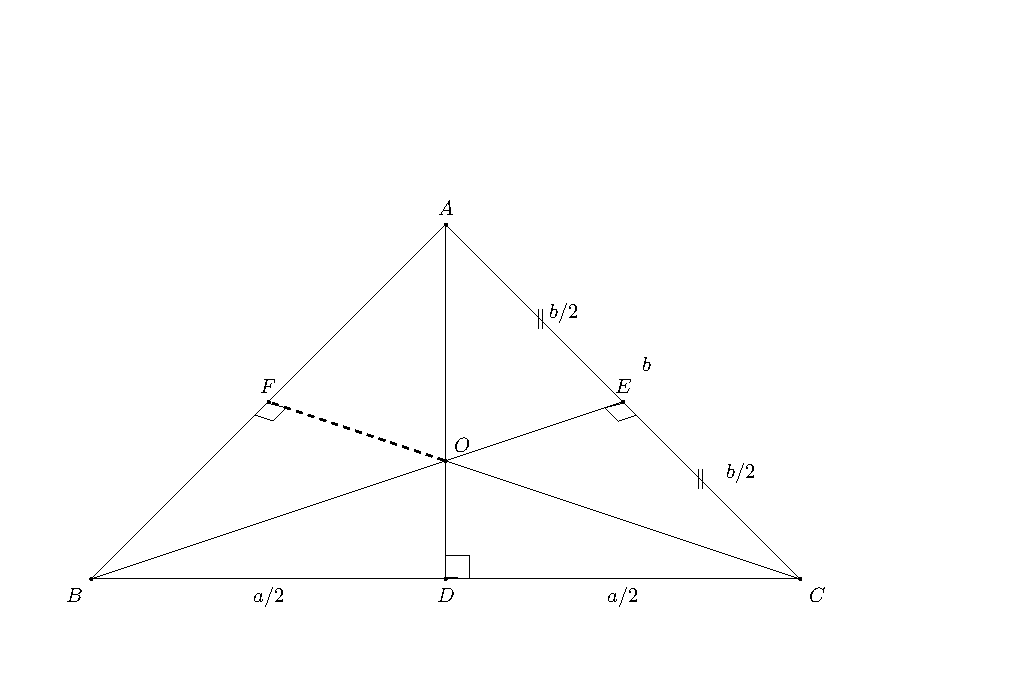
\includegraphics[width=\columnwidth]{./figs/fig_3.8.eps}
%%		\includegraphics[width=\columnwidth]{./figs/ch3_perp_bisector}
%		%\vspace*{-10cm}
%%		\resizebox{\columnwidth}{!}{\documentclass{standalone}
\usepackage{tikz}
\usepackage{tkz-euclide}
\usetkzobj{all}
%\usepackage{amsmath}
\providecommand{\brak}[1]{\ensuremath{\left(#1\right)}}

\begin{document}
\begin{tikzpicture}
[scale=2,>=stealth,point/.style={draw,circle,fill = black,inner sep=0.5pt},]

\node (E) at (1.5, 1.5)[point,label=above :$E$] {};
\node (F) at (-1.5, 1.5)[point,label=above :$F$] {};
\node (A) at (0, 3)[point,label=above :$A$]{};
\node (B) at (-3, 0)[point,label=below left:$B$]{};
\node (C) at (3, 0)[point,label=below right:$C$]{};
\node (D) at (0,0)[point,label=below :$D$] {};
\node (O) at (0,1)[point,label=above right :$O$] {};


\draw (B)--(A);
\draw (A)--(C);
\draw (B)--(C);
\draw (B)--(E);
\draw (C)--(O);
\draw (A)--(D);
\draw [thick,dashed] (O) -- (F);

\node [above] at (1.7,1.7) {$b$};
\node [above] at (2.5,.75) {$b/2$};
\node [above] at (1,2.1) {$b/2$};
\node [above] at (-1.5,-0.3){$a/2$};
\node [above] at (1.5,-0.3){$a/2$};
\tkzMarkRightAngle[size=.16](B,F,O)
\tkzMarkRightAngle[size=.16](C,E,O)
\tkzMarkRightAngle[size=.2](A,D,C)
\draw   -- (4.3,1.7) node[midway] {$\parallel$};
\draw   -- (1.6,4.4) node[midway] {$\parallel$};

\end{tikzpicture}
\end{document}}
%	\end{center}
%	\caption{Perpendicular bisectors meet at a point}
%	\label{ch3_perp_bisector}	
%\end{figure}
%%
%\solution In $\Delta$s $ODB$ and $ODC$, using Budhayana's theorem,
%%
%\begin{equation}
%\begin{split}
%OB^2 &= OD^2 + BD^2 \\
%OC^2 &= OD^2 + DC^2 
%\end{split}
%\end{equation}
%%
%Since $BD = DC = \frac{a}{2}$, $OB = OC$.  Similarly, it can be shown that $OA = OC$.  Thus, $OA=OB=OC$.
%%
%\item
%	In $\Delta AOB$, $OA = OB$.  Such a triangle is known as an isoceles triangle.
%
%%
%\item
%	Show that $AF = BF$.
%
%\solution Trivial using Budhayana's theorem.  This shows that $OF$ is a perpendicular bisector of $AB$. 
%{\em Conclusion:}  The perpendicular bisectors of a triangle meet at a point.
%%
%\end{enumerate}
%
%\subsection{Perpendiculars from Vertex to Opposite Side}
%\renewcommand{\theequation}{\theenumi}
%\begin{enumerate}[label=\arabic*.,ref=\thesubsection.\theenumi]
%\numberwithin{equation}{enumi}
%	%
%	%
%\item
%	In Fig. \ref{ch3_perp_triang}, $AD \perp BC$ and $BE \perp AC$. $CF$ passes through $O$ and meets
%	$AB$ at $F$.  	
%	Show that 
%	\begin{align}
%	OE = c \cos A \cot C
%	\end{align}
%
%	\begin{figure}[!ht]
%		\begin{center}
%			
%			%\includegraphics[width=\columnwidth]{./figs/ch3_perp_triang}
%			%\vspace*{-10cm}
%			\resizebox{\columnwidth}{!}{\begin{tikzpicture}
[scale=2,>=stealth,point/.style={draw,circle,fill = black,inner sep=0.5pt},]

\node (E) at (1.5, 1.5)[point,label=above :$E$] {};
\node (F) at (-1.5, 1.5)[point,label=above :$F$] {};
\node (A) at (0, 3)[point,label=above :$A$]{};
\node (B) at (-3, 0)[point,label=below left:$B$]{};
\node (C) at (3, 0)[point,label=below right:$C$]{};
\node (O) at (0,1)[point,label=above right :$O$] {};
\node (D) at (0,0)[point,label=below :$D$] {};


\draw (B)--(A);
\draw (A)--(C);
\draw (B)--(E);
\draw (C)--(F);
\draw (B)--(C);
\draw (A)--(D);

\node [below] at (0,-0.3) {$a$};
\node [above] at (-1.7,1.7) {$c$};
\node [above] at (1.7,1.7) {$b$};
\node [above] at (1,1.3) {$p$};
\node [above] at (-1,1.3) {$q$};
\node [above] at (-2.3,0.24){\rotatebox{45}{$90-A$}};
\node [above] at (-0.4,2.1) {\rotatebox{45}{$90-B$}};
\node [above] at (0.4,2.1) {\rotatebox{-45}{$90-C$}};

\tkzMarkAngle[size=.3](F,O,B);
\tkzMarkAngle[size=.3](C,O,E);
\tkzMarkAngle[size=.4](O,B,F);
\tkzMarkAngle[size=.2](F,A,O);
\tkzMarkAngle[size=.3](O,A,E);
\draw (-0.5,1) node{$\alpha$};
\draw (0.5,1) node{$\alpha$};

\end{tikzpicture}
}
%		\end{center}
%		\caption{Perpendiculars from vertex to opposite side meet at a point}
%		\label{ch3_perp_triang}	
%	\end{figure}
%%
%\solution In $\Delta$ s $AEB$ and $AEO$,
%%
%\begin{align}
%AE &= c \cos A \\
%OE &= AE \tan \brak{90^{\degree} - C} \brak{\because ADC \text{ is right angled}} \\
%&= AE \cot C
%\end{align}
%%
%From both the above, we get the desired result.
%%
%\item
%	Show that $\alpha = A$.
%
%\solution In $\Delta OEC$,
%%
%\begin{equation}
%CE = a \cos C \brak{\because BEC \text{ is right angled}}
%\end{equation}
%%
%Hence,
%%
%\begin{equation}
%\begin{split}
%\tan \alpha &= \frac{CE}{OE} \\
%&=  \frac{a \cos C}{c \cos A \cot C} \\
%&=  \frac{a \cos C \sin C}{c \cos A \cos C} \\
%&= \frac{a \sin C}{c \cos A } \\
%&= \frac{c \sin A}{c \cos A } \brak{\because \frac{a}{\sin A} = \frac{c}{\sin C}}\\
%&= \tan A\\
%\Rightarrow \alpha = A
%\end{split}
%\end{equation}
%%
%\item
%	Show that $CF \perp AB$
%
%\solution Consider triangle OFB and the result of the previous problem.  $\because$ the sum of the angles of a triangle is $180^{\degree}$, $\angle CFB = 90^{\degree}$.
%{\em Conclusion: The perperdiculars from the vertex of a triangle to the opposite side meet at a point.}
\end{enumerate}
